% XeLaTeX document
\documentclass[12pt,a4paper]{article}

% Редактируем: конфигурация, личные настройки: имя, название предмета и пр. для титульной страницы и метаданных документа здесь
\newcommand{\university}{Национальный исследовательский Университет ИТМО}
\newcommand{\mfaculty}{Мегафакультет информационных и трансляционных технологий}
\newcommand{\faculty}{Факультет инфокоммуникационных технологий}
\newcommand{\city}{Санкт-Петербург}
\newcommand{\num}{ №7}
\newcommand{\docname}{Лабораторная работа}
\newcommand{\subject}{Алгоритмы и структуры данных}
\newcommand{\tutorname}{Артамонова В.Е.}
\newcommand{\studentname}{Рудникова В.О.}
\newcommand{\group}{К3125}

% Не редактируем: используемые пакеты
% настройка кодировки, шрифтов и русского языка
\usepackage{fontspec}
\usepackage{polyglossia}

% рабочие ссылки в документе
\usepackage{hyperref}

% графика
\usepackage{graphicx}
\usepackage{tikz}

% поворот страницы
\usepackage{pdflscape}

% качественные листинги кода
\usepackage{minted}
\usepackage{listings}
\usepackage{lstfiracode}

% отключение копирования номеров строк из листинга, работает не во всех просмотрщиках (в Adobe Reader работает)
\usepackage{accsupp}
\newcommand\emptyaccsupp[1]{\BeginAccSupp{ActualText={}}#1\EndAccSupp{}}
\let\theHFancyVerbLine\theFancyVerbLine
\def\theFancyVerbLine{\rmfamily\tiny\emptyaccsupp{\arabic{FancyVerbLine}}}

% библиография
\bibliographystyle{templates/gost-numeric.bbx}
\usepackage{csquotes}
\usepackage[parentracker=true,backend=biber,hyperref=true,bibencoding=utf8,style=numeric-comp,language=auto,autolang=other,citestyle=gost-numeric,defernumbers=true,bibstyle=gost-numeric,sorting=ntvy]{biblatex}

% установка полей
\usepackage{geometry}

% нумерация картинок по секциям
\usepackage{chngcntr}

% дополнительные команды для таблиц
\usepackage{booktabs}

% для заголовков
\usepackage{caption}
\usepackage{titlesec}
\usepackage[dotinlabels]{titletoc}

% разное для математики
\usepackage{amsmath, amsfonts, amssymb, amsthm, mathtools}

% водяной знак на документе, см. main.tex
\usepackage[printwatermark]{xwatermark}

% Не редактируем: параметры используемых пакетов и не только
% настройки polyglossia
\setdefaultlanguage{russian}
\setotherlanguage{english}

% локализация
\addto\captionsrussian{
	\renewcommand{\figurename}{Рисунок}%
	\renewcommand{\partname}{Глава}
	\renewcommand{\contentsname}{\centerline{Содержание}}
	\renewcommand{\listingscaption}{Листинг}
}

% основной шрифт документа
\setmainfont{CMU Serif}
\newfontfamily\cyrillicfont{CMU Serif}[Script=Cyrillic]

% перечень использованных источников
\addbibresource{refs.bib}

% настройка полей
\geometry{top=2cm}
\geometry{bottom=2cm}
\geometry{left=2cm}
\geometry{right=2cm}
\geometry{bindingoffset=0cm}

% настройка ссылок и метаданных документа
\hypersetup{unicode=true,colorlinks=true,linkcolor=red,citecolor=green,filecolor=magenta,urlcolor=cyan,
	pdftitle={\docname},
	pdfauthor={\studentname},
	pdfsubject={\subject},
	pdfcreator={\studentname},
	pdfproducer={Overleaf},
	pdfkeywords={\subject}
}

% настройка подсветки кода и окружения для листингов
\usemintedstyle{colorful}
\newenvironment{code}{\captionsetup{type=listing}}{}

% шрифт для листингов с лигатурами
\setmonofont{FiraCode-Regular.otf}[
	SizeFeatures={Size=10},
	Path = templates/,
	Contextuals=Alternate
]

% оформления подписи рисунка
\captionsetup[figure]{labelsep = period}

% подпись таблицы
\DeclareCaptionFormat{hfillstart}{\hfill#1#2#3\par}
\captionsetup[table]{format=hfillstart,labelsep=newline,justification=centering,skip=-10pt,textfont=bf}

% путь к каталогу с рисунками
\graphicspath{{fig/}}

% Внесение titlepage в учёт счётчика страниц
\makeatletter
\renewenvironment{titlepage} {
	\thispagestyle{empty}
}
\makeatother

\counterwithin{figure}{section}
\counterwithin{table}{section}

\titlelabel{\thetitle.\quad}

% для удобного конспектирования математики
\mathtoolsset{showonlyrefs=true}
\theoremstyle{plain}
\newtheorem{theorem}{Теорема}[section]
\newtheorem{proposition}[theorem]{Утверждение}
\theoremstyle{definition}
\newtheorem{corollary}{Следствие}[theorem]
\newtheorem{problem}{Задача}[section]
\theoremstyle{remark}
\newtheorem*{nonum}{Решение}

% настоящее матожидание
\newcommand{\MExpect}{\mathsf{M}}

% объявили оператор!
\DeclareMathOperator{\sgn}{\mathop{sgn}}

% перенос знаков в формулах (по Львовскому)
\newcommand*{\hm}[1]{#1\nobreak\discretionary{} {\hbox{$\mathsurround=0pt #1$}}{}}


% водяной знак для обозначения статуса документа
%\newwatermark[allpages,color=red!5,angle=45,scale=3,xpos=0,ypos=0]{DRAFT}
\begin{document}
% Не редактируем: Титульная страница (формируется автоматически из заданной конфигурации)
\begin{titlepage}	% начало титульной страницы

	\begin{center}		% выравнивание по центру

		\large \university \\
		\large \mfaculty \\
		\large \faculty \\[6cm]
		% название института, затем отступ 6см

		\huge \subject \\[0.5cm] % название работы, затем отступ 0,5см
		\large \docname  \num \\[5.1cm]
		 %\large Разработка методов обучения с подкреплением\\[5cm]

	\end{center}


	\begin{flushright} % выравнивание по правому краю
		\begin{minipage}{0.25\textwidth} % врезка в половину ширины текста
			\begin{flushleft} % выровнять её содержимое по левому краю

				\large\textbf{Работу выполнил:}\\
				\large \studentname \\
				\large {Группа:} \group \\

				\large \textbf{Преподаватель:}\\
				\large \tutorname

			\end{flushleft}
		\end{minipage}
	\end{flushright}

	\vfill % заполнить всё доступное ниже пространство

	\begin{center}
		\large \city \\
		\large \the\year % вывести дату
	\end{center} % закончить выравнивание по центру

\end{titlepage} % конец титульной страницы

\vfill % заполнить всё доступное ниже пространство


% Не редактируем: Страница содержания (формируется автоматически из section, subsection и пр., указанных в content.tex)
% Содержание
\tableofcontents
\newpage



% Редактируем: всё остальное: вступление, др. этапы, заключение, приложение
\section*{Задачи по варианту}
\addcontentsline{toc}{section}{Задачи по варианту}




\subsection*{Задача 4. Наибольшая общая подпоследовательность двух последовательностей}
\addcontentsline{toc}{subsection}{Задача 4. Наибольшая общая подпоследовательность двух последовательностей}

Вычислить длину самой длинной общей подпоследовательности из двух
последовательностей. Даны две последовательности: $A = (a_1, a_2, ..., a_n)$ и $B = (b_1, b_2, ..., b_m)$, найти длину их самой длинной общей
подпоследовательности, т.е. наибольшее неотрицательное целое число $p$
такое, что существуют индексы $ 1 \le i_1 < i_2 < ... < i_p \le n$ и $ 1 \le j_1 < j_2 < ... < j_p \le m $ такие, что $ a_{i1} = b_{j1}, ..., a_{ip} = b_{jp}. $

\begin{itemize}
    \item Формат ввода / входного файла (input.txt).
    \newline – Первая строка: $n$ - длина первой последовательности.
    \newline – Вторая строка: $a_1, a_2, ..., a_n$ через пробел.
    \newline – Третья строка: $m$ - длина второй последовательности.
    \newline – Четвертая строка: $b_1, b_2, ..., b_m$ через пробел.
    \item Ограничения: $1 \le n, m \le 100; −10^9 < a_i, b_i < 10^9$.
    \item Формат вывода / выходного файла (output.txt). Выведите число $p$.
    \item Ограничение по времени. 1 сек.
\end{itemize}
\addcontentsline{toc}{subsubsection}{Условие задачи}

\begin{code}
	\inputminted[breaklines=true, xleftmargin=1em, linenos, frame=single, framesep=10pt, fontsize=\footnotesize, firstline=1, lastline=29]{python}{listings/task4.py}
\end{code}
\addcontentsline{toc}{subsubsection}{Листинг кода}
\newline
Длина общих подпоследовательностей хранится в двумерном списке,
каждая мера которого отвечает за одну из данных последовательностей.
Длина общей подпоследовательности для каждой ячейки списка
определяется его предыдущими ячейками.
\addcontentsline{toc}{subsubsection}{Текстовое объяснение решения}

\newpage
Результат работы кода на примерах из текста задачи:\ref{pic4}
\begin{figure}[H]
    \label{pic4}
	\begin{center}
		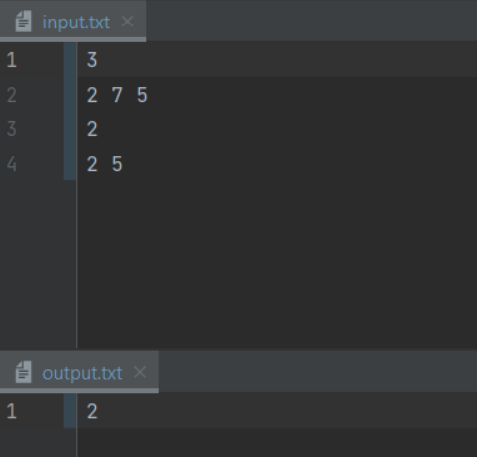
\includegraphics[scale=0.7]{fig/4_text.png}
	\end{center}
\end{figure}
\newline
Результат работы кода на минимальных и максимальных значениях:\ref{pic3}
\begin{figure}[H]
        \label{pic3}
	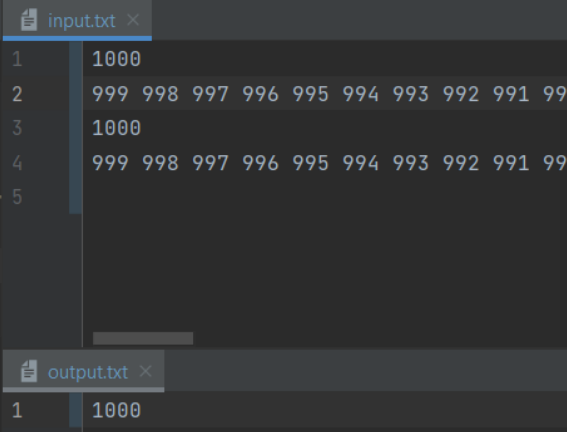
\includegraphics[scale=0.7]{fig/4_max.png}
	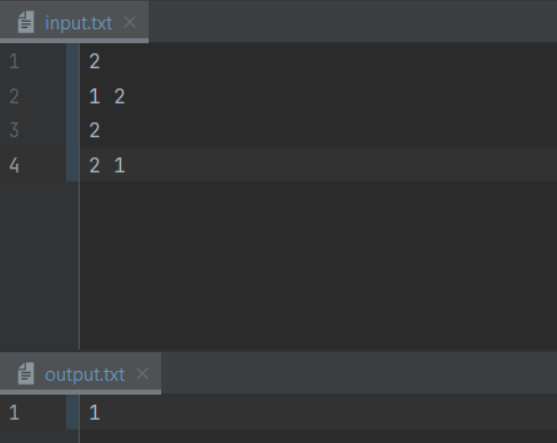
\includegraphics[scale=0.7]{fig/4_min.png}
\end{figure}
\addcontentsline{toc}{subsubsection}{Результаты работы кода}

\newpage
\begin{table}[]
    \begin{center}
        \begin{tabular}{|l|l|l|}
        \hline
             & Время выполнения & Затраты памяти  \\ \hline
            \begin{tabular}[c]{@{}l@{}}Нижняя граница\\ диапазона значений\\ входных данных из\\ текста задачи\end{tabular}  &  0.078375 seс  &  17.244140625 KB \\ \hline
            Пример из задачи  &  0.078375 sec  &  17.244140625 KB \\ \hline
            \begin{tabular}[c]{@{}l@{}}Верхняя граница\\ диапазона значений\\ входных данных из\\ текста задачи\end{tabular} & 0.078375 sec  & 17.244140625 KB \\ \hline
        \end{tabular} 
    \end{center}
\end{table}
\addcontentsline{toc}{subsubsection}{Время выполнения и затраты памяти}

\newline
\textbf{Вывод по задаче:} \newline
В задаче я реализовала алгоритм поиска длины наибольшей общей подпоследовательности для двух последовательностей.
\cite{wiki}
\addcontentsline{toc}{subsubsection}{Вывод по задаче}







\newpage
\section*{Дополнительные задачи}
\addcontentsline{toc}{section}{Дополнительные задачи}

\subsection*{Задача 5. Наибольшая общая подпоследовательность трёх последовательностей}
\addcontentsline{toc}{subsection}{Задача 5. Наибольшая общая подпоследовательность трёх последовательностей}

Вычислить длину самой длинной общей подпоследовательности из двух
последовательностей. Даны три последовательности: $A = (a_1, a_2, ..., a_n)$, $B = (b_1, b_2, ..., b_m)$ и $C = (c_1, c_2, ..., c_k)$ найти длину их самой длинной общей
подпоследовательности, т.е. наибольшее неотрицательное целое число $p$
такое, что существуют индексы $ 1 \le i_1 < i_2 < ... < i_p \le n$, $ 1 \le j_1 < j_2 < ... < j_p \le m $ и $ 1 \le k_1 < k_2 < ... < k_p \le n$ такие, что $ a_{i1} = b_{j1} = c_{k1}, ..., a_{ip} = b_{jp}  c_{kp}.

\begin{itemize}
    \item Формат ввода / входного файла (input.txt).
    \newline – Первая строка: $n$ - длина первой последовательности.
    \newline – Вторая строка: $a_1, a_2, ..., a_n$ через пробел.
    \newline – Третья строка: $m$ - длина второй последовательности.
    \newline – Четвертая строка: $b_1, b_2, ..., b_m$ через пробел.
    \newline – Пятая строка: $k$ - длина третьей последовательности.
    \newline – Шестая строка: $cс_1, c_2, ..., c_k$ через пробел.
    \item Ограничения: $1 \le n, m \le 100; −10^9 < a_i, b_i < 10^9$.
    \item Формат вывода / выходного файла (output.txt). Выведите число $p$.
    \item Ограничение по времени. 1 сек.\eqref{eq:eq1}
\end{itemize}
\addcontentsline{toc}{subsubsection}{Условие задачи}



\newline
\begin{equation}
    \centering
    \label{eq:eq1}
        y = \frac{x^2-3}{x-2}.
\end{equation}
\newpage
\begin{code}
	\inputminted[breaklines=true, xleftmargin=1em, linenos, frame=single, framesep=10pt, fontsize=\footnotesize, firstline=1, lastline=34]{python}{listings/task5.py}
\end{code}
\addcontentsline{toc}{subsubsection}{Листинг кода}
\newline
Длина общих подпоследовательностей хранится в трёхмерном списке,
каждая мера которого отвечает за одну из данных последовательностей.
Длина общей подпоследовательности для каждой ячейки списка
определяется его предыдущими ячейками. \newline
\addcontentsline{toc}{subsubsection}{Текстовое объяснение решения}

\newpage
Результат работы кода на примерах из текста задачи:\ref{pic1}
\begin{figure}[H]
        \label{pic1}
	\begin{center}
		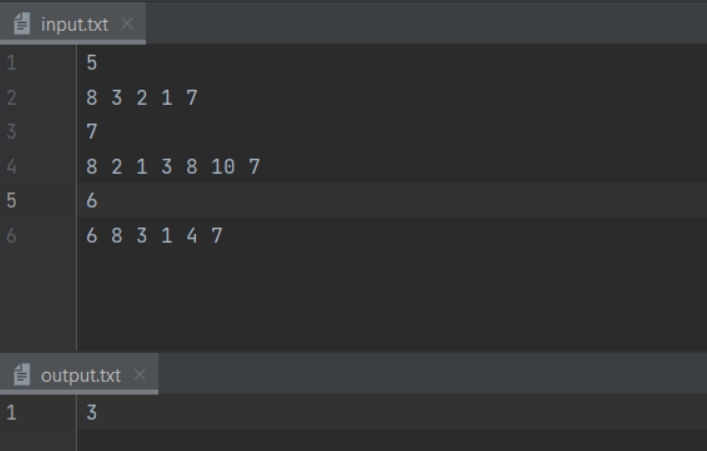
\includegraphics[scale=0.7]{fig/5_text.png}
	\end{center}
\end{figure}
\newline
Результат работы кода на минимальных и максимальных значениях:\ref{pic2}
\begin{figure}[H]
        \label{pic2}
	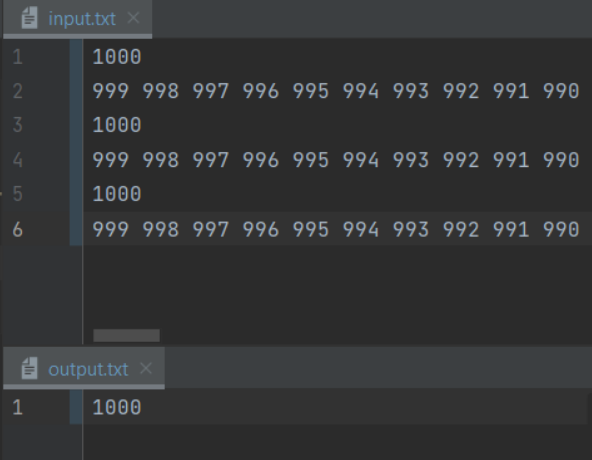
\includegraphics[scale=0.7]{fig/5_max.png}
	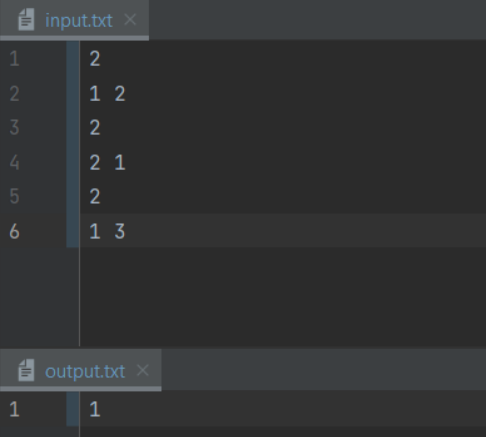
\includegraphics[scale=0.7]{fig/5_min.png}
\end{figure}
\addcontentsline{toc}{subsubsection}{Результаты работы кода}

\newpage
\begin{table}[]
    \begin{center}
        \begin{tabular}{|l|l|l|}
        \hline
             & Время выполнения & Затраты памяти  \\ \hline
            \begin{tabular}[c]{@{}l@{}}Нижняя граница\\ диапазона значений\\ входных данных из\\ текста задачи\end{tabular}  &  0.078375 seс  &  17.244140625 KB \\ \hline
            Пример из задачи  &  0.078375 sec  &  17.244140625 KB \\ \hline
            \begin{tabular}[c]{@{}l@{}}Верхняя граница\\ диапазона значений\\ входных данных из\\ текста задачи\end{tabular} & 0.078375 sec  & 17.244140625 KB \\ \hline
        \end{tabular} 
    \end{center}
\end{table}
\addcontentsline{toc}{subsubsection}{Время выполнения и затраты памяти}

\newline
\textbf{Вывод по задаче:} \newline
В задаче я реализовала алгоритм поиска длины наибольшей общей подпоследовательности для трёх последовательностей.
\addcontentsline{toc}{subsubsection}{Вывод по задаче}








\newpage
\section*{Вывод:}
\addcontentsline{toc}{section}{Вывод}
В работе я вспомнила принципы динамического программирования и их
применение к задачам про общие подпоследовательности.
\newline
\newline


% Не редактируем: Страница библиографии (формируется автоматически из книжек, указанных в refs.bib и пометок \cite{имя_источника} в тексте)
\newpage
\printbibliography[title=Список использованных источников]
\addcontentsline{toc}{section}{Список использованных источников}
\end{document}
